\subsection{Pruebas unitarias.}

Las pruebas unitarias constituyen un componente fundamental en cualquier proceso de desarrollo de software moderno. Son el primer nivel de pruebas que se realizan para validar la funcionalidad de las unidades más pequeñas del código, como funciones o métodos individuales.

Se desarrollaron pruebas unitarias específicas que cubren los casos de uso que encapsulan la lógica de negocio principal (operaciones con los datos, CRUD). La estrategia de testing adoptada utilizó \texttt{JUnit 4} como framework base y \texttt{mockk} para simluar las entidades usadas en la aplicación real.Los resultados de las pruebas se muestran en la Figura \ref{fig:resultados_pruebas_unitarias}. 

\begin{figure}[ht!]
  \captionof{figure}{Resultados pruebas unitarias.}
  \label{fig:resultados_pruebas_unitarias}
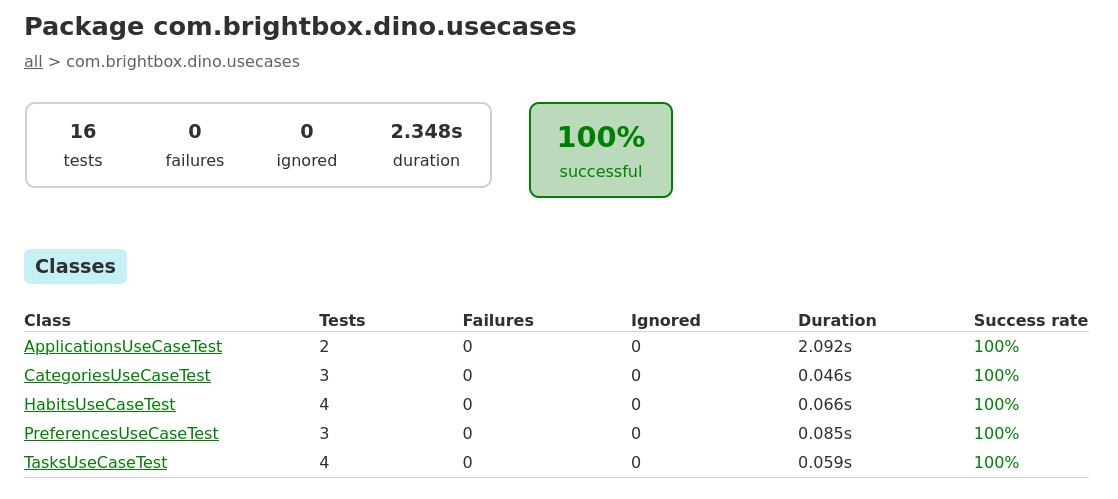
\includegraphics[width=\textwidth]{Figuras/resultados_pruebas_unitarias.png}
  \centering
\end{figure}